\chapter{Realisierung des IIR-Filters}\label{Cha:RealIIR}
\section{Aufgabenstellung}
Die Aufgabe dieser Übung bestand darin, einen IIR Filter zu realisieren. Dabei galt besonderes Augenmerk der Minimierung von Rundungsfehlern sowie der Verhinderung von Überläufen.
\section{Durchf\"uhrung}
Das Filter wird auf die nachfolgenden vier Varianten implementiert. Vorab wurden dazu die Filterkoeffizienten entsprechend der Aufgabe nach aufsteigendem Radius im Einheitskreis sortiert.

Es wurden wie in der Aufgabe beschrieben die Dateien in ein neues Projekt eingefügt und wie im folgenden beschrieben entsprechend angepasst.
\subsection{Skalierung am Eingang}
Die einfachste Form der Skalierung ist die Skalierung am Eingang, wobei mit einem Diviesor vor verwenden des Filters dividiert wird. Dazu wird zuerst die gesamte Verstärkung der Filter durch Multiplikation ermittelt.
Da es sich um einen Tiefpass handelt wird die Verstärkung bei 0Hz berechnet. Es folgt: z=1.
Gemäß folgender Formel ergibt sich eine Gesamtverstärkung von 474.5917.
\begin{equation}
\Pi H_i(1)=1,355*1,891*4,866*38,3=474.5917
\end{equation}
Todo:  robby bitte die werte anpassen so dass die rechnung stimmt hier stimmt nur das ergebnis mit unserem sourcecode überein.
Daraus folgt die Anpassung der Datei process\textunderscore data.c wie folgt.\\

\begin{adjustbox}{width=\textwidth,height=\textheight,keepaspectratio}
 \begin{lstlisting}[title=processdata.c]{processdata.c}
// Definition der Filterkoeffizienten
#define BIQUAD_STAGES 4

// coef includes for all stages a scaling factor (2^s) and five coefficients
// in the order s, b2, b1, b0, a2, a1

// No scaling in stages (Low Pass)
const short coef[6*BIQUAD_STAGES] = {
	1, 16384, 6581	, 16384, -10390, 25748  //H4
	1, 16384, -20909, 16384, -12529, 26454, //H3
	1, 16384, -25583, 16384, -14605, 27191, //H2
	1, 16384, -26706, 16384, -15896, 27808, //H1
};

int iDelayline[2*BIQUAD_STAGES+2];	// delayline for left and right channel samples

IIRstateStereo iirLR={coef,iDelayline,BIQUAD_STAGES};

void process_data()
{
	//!! Scale before filtering
	sADC1L = sADC1L / 474.5917; //skalierungsfaktor aus Rechnung
	sADC1R = sADC1R / 474.5917;
	*(int*)(&sDAC1L) = iir_stereo(*(int*)(&sADC1L),&iirLR);

	//!! Scale after filtering
}
\end{lstlisting}
\end{adjustbox}
Die Interprätierung als 1.15 Format findet sich in den eingetragenen Koeffizienten nicht, sie wurden als short implementiert. Die Konvertierung erfolgte wie in früheren Laborübungen gesehen. Die Implementierung als short ermöglicht eine bessere Übersichtlichkeit und vermeidet Fehler. Die Zweite Anpassung war die eigentliche Skalierung am Eingang, hierzu wurde der zuvor ermittelte Divisor verwendet.\\
\begin{figure}[H]
  \centering
    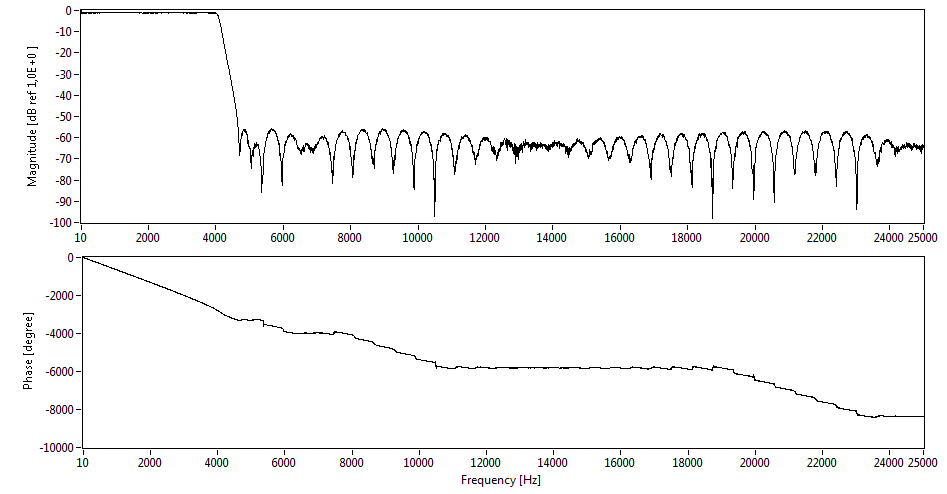
\includegraphics[width=\textwidth]{Freqgang3_1.png}
  \caption{Frequenzgang}
  \label{fig:Freqgang3_1}
\end{figure}
Hier wurde der Frequenzgang des Systems visualisiert, es ist deutlich das Tiefpassverhalten auszumachen. Die Grenzfrequenz liegt bei etwa 4kHz.\\
Zur weiteren Untersuchung wurde folgendes Sinussignal mit 2kHz Frequenz und 50mV Amplitude eingespeist.
\begin{figure}[H]
  \centering
    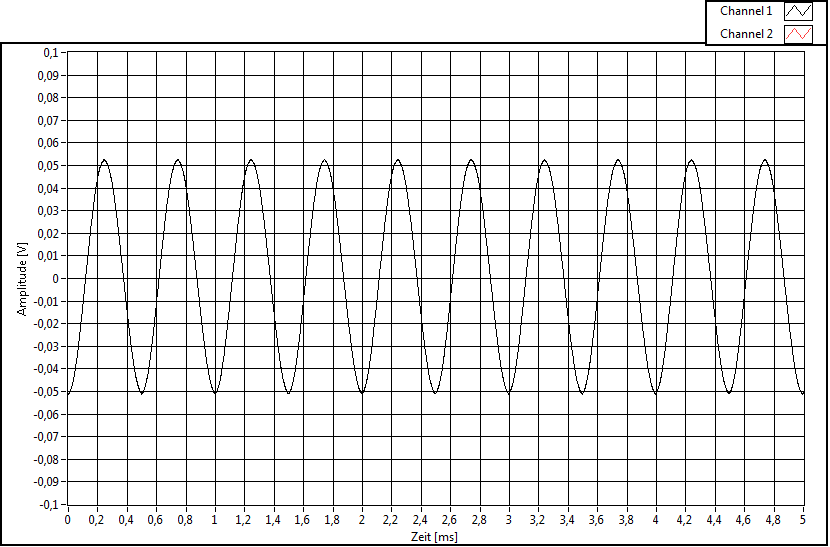
\includegraphics[width=\textwidth]{Eingangssignal50mv2kHz.png}
  \caption{Eingangssignal}
  \label{fig:Eingangssignal50mv2kHz}
\end{figure}
Wir haben am Eingang das nachfolgende Spektrum gemessen.
\begin{figure}[H]
  \centering
    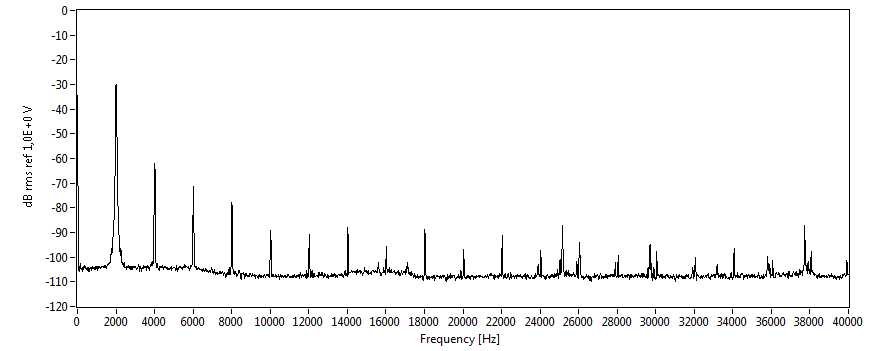
\includegraphics[width=\textwidth]{PowerspekEingang.png}
  \caption{Spektrum am Eingang}
  \label{fig:PowerspekEingang}
\end{figure}
Und am Ausgang hat man in nachstehendem Spektrum das Rauschen gut beobachten können.
\begin{figure}[H]
  \centering
    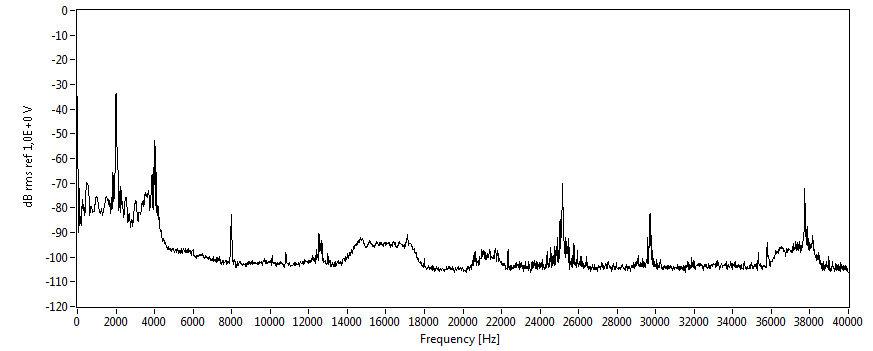
\includegraphics[width=\textwidth]{PowerspekAusgang.png}
  \caption{Spektrum am Ausgang}
  \label{fig:PowerspekAusgang}
\end{figure}
Es ist gut zu sehen, dass am Eingang mehrere Harmonische alle 2kHz zu sehen sind, umgeben von einem sehr geringen Rauschteppich bei unter -100dB. Am Ausgang hingegen ist das Tiefpassverhalten zu erkennen, was die erste Harmonische bei 4kHz (der Grenzfrequenz) noch leicht gedämpft darstellt, alle weiteren Harmonischen aber hinreichend unterdrückt. Außerdem lässt sich ein Rauschen ausmachen, was bis zur Grenzfrequenz um -80dB liegt. Dieses Bild entspricht unseren Erwartungen.
\subsection{Skalierung am Ausgang}
Entsprechend der Aufgabenstellung haben wir auch die Skalierung am Ausgang umgesetzt, wie erwartet übersteuerte das System massiv, was die Analyse der Implementierungsvariante unnütz machte. Aus diesem Grund verzichten wir wie Abgesprochen auf eine Auswertung an dieser Stelle.
\subsection{Gleichmäßige Skalierung}
Im dritten Teil der Übung wurde das Filter gleichmäßig über alle Teilfilter skaliert. Dazu wurde die Gesamtverstärkung aus dem ersten Teil gleichmäßig auf die Teilfilter aufgteteilt. Der Divisor ergibt sich also wie folgt:\\
\begin{equation}
\sqrt[4]{474.5917}=4,6675
\end{equation}

\begin{adjustbox}{width=\textwidth,height=\textheight,keepaspectratio}
 \begin{lstlisting}[title=processdata.c]
 
 // No scaling in stages (Low Pass)
const short coef[6*BIQUAD_STAGES] = {
	1, 3514, 1412, 3514, -2229, 5523, //H4
	1, 3514, -4485, 3514, -2687, 5674,//H3
	1, 3514, -5488, 3514, -3133, 5832,//H2
	1, 3514, -5728, 3514, -3410, 5965 //H1
};



int iDelayline[2*BIQUAD_STAGES+2];	// delayline for left and right channel samples

IIRstateStereo iirLR={coef,iDelayline,BIQUAD_STAGES};

void process_data()
{
	//!! Scale before filtering
	*(int*)(&sDAC1L) = iir_stereo(*(int*)(&sADC1L),&iirLR);
	//!! Scale after filtering

}
\end{lstlisting}
\end{adjustbox}
\begin{figure}[H]
  \centering
    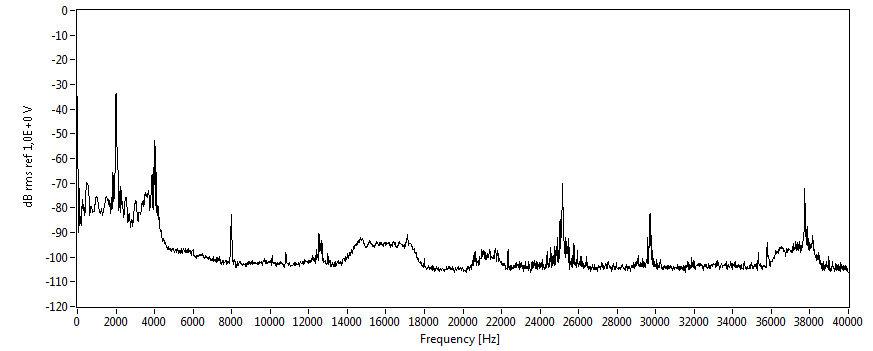
\includegraphics[width=\textwidth]{PowerspekAusgang.png}
  \caption{Spektrum am Ausgang}
  \label{fig:PowerspekAusgang}
\end{figure}
\begin{figure}[H]
  \centering
    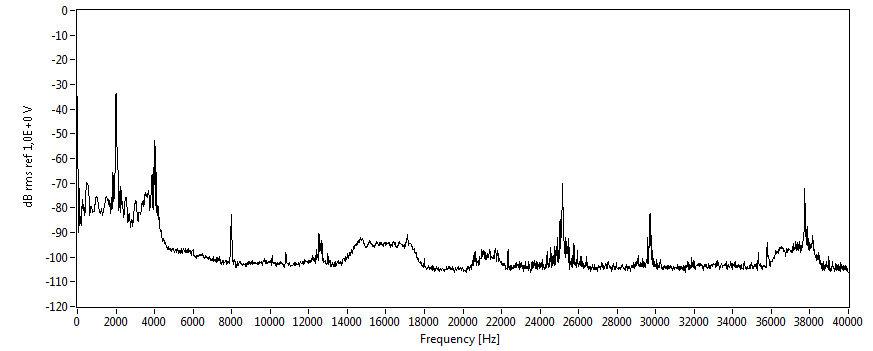
\includegraphics[width=\textwidth]{PowerspekAusgang.png}
  \caption{Spektrum am Ausgang}
  \label{fig:PowerspekAusgang}
\end{figure}
\begin{figure}[H]
  \centering
    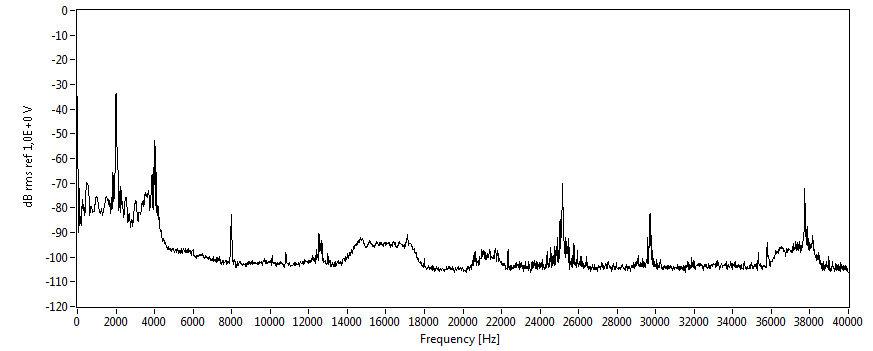
\includegraphics[width=\textwidth]{PowerspekAusgang.png}
  \caption{Spektrum am Ausgang}
  \label{fig:PowerspekAusgang}
\end{figure}
\begin{figure}[H]
  \centering
    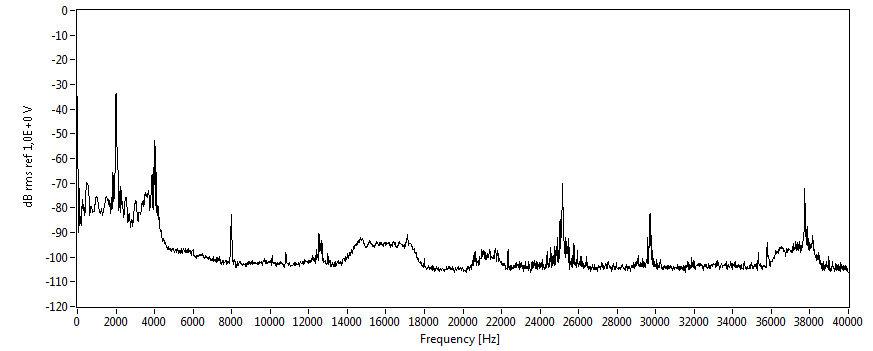
\includegraphics[width=\textwidth]{PowerspekAusgang.png}
  \caption{Spektrum am Ausgang}
  \label{fig:PowerspekAusgang}
\end{figure}
\begin{figure}[H]
  \centering
    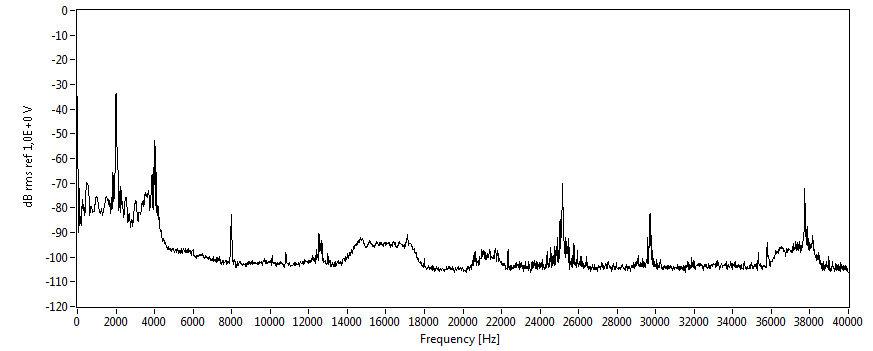
\includegraphics[width=\textwidth]{PowerspekAusgang.png}
  \caption{Spektrum am Ausgang}
  \label{fig:PowerspekAusgang}
\end{figure}
\begin{figure}[H]
  \centering
    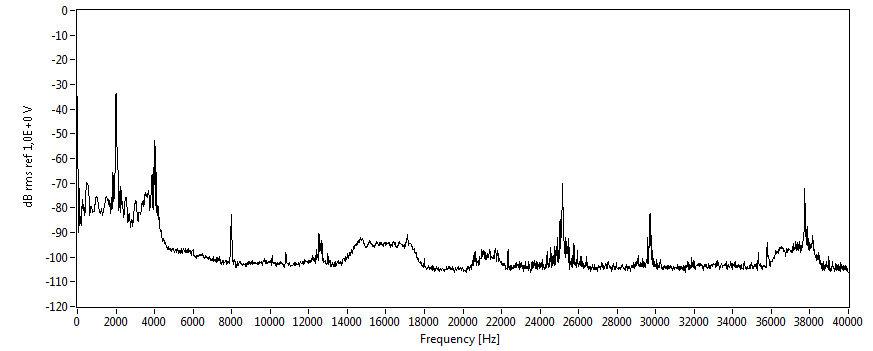
\includegraphics[width=\textwidth]{PowerspekAusgang.png}
  \caption{Spektrum am Ausgang}
  \label{fig:PowerspekAusgang}
\end{figure}
\subsection{Optimierte Skalierung}
\section{Auswertung}
